\documentclass[border=0.8ex,svgnames,tikz]{standalone}
\usepackage{amsmath,mathtools}
\usepackage{fontspec}
\setmainfont{Source Serif 4}
\setsansfont{Source Sans 3}
\setmonofont{Source Code Pro}
\usetikzlibrary{positioning,calc}
\begin{document}
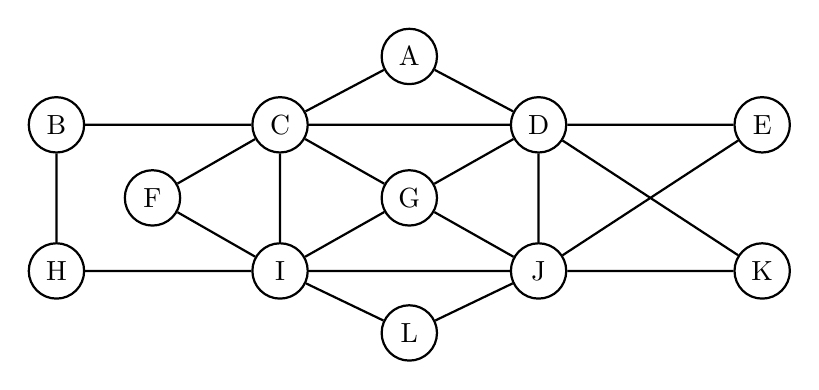
\begin{tikzpicture}[
  node distance=2em,
  every node/.style={draw,circle,minimum size=2em},
  every path/.style={draw,>=latex,thick},
  ]
  \coordinate(graph);
  \node[below=of graph] (graphA) {A};
  \node[below left=1em and 3.2em of graphA] (graphC) {C};
  \node[left=6em of graphC] (graphB) {B};
  \node[below right=1em and 3.2em of graphA] (graphD) {D};
  \node[right=6em of graphD] (graphE) {E};
  \node[below=1.6em of $(graphC)!0.5!(graphD)$] (graphG) {G};
  \node[left=7.2em of graphG] (graphF) {F};
  \node[below=3.2em of graphC] (graphI) {I};
  \node[left=6em of graphI] (graphH) {H};
  \node[below=3.2em of graphD] (graphJ) {J};
  \node[right=6em of graphJ] (graphK) {K};
  \node[below=1.2em of $(graphI)!0.5!(graphJ)$] (graphL) {L};
  \path
  (graphE) -- (graphD) -- (graphA) -- (graphC) -- (graphB) -- (graphH) -- (graphI) --
  (graphL) -- (graphJ) -- (graphI) -- (graphF) -- (graphC) -- (graphG) -- (graphD) --
  (graphK) -- (graphJ) -- (graphG) -- (graphI) -- (graphC) -- (graphD) -- (graphJ) --
  (graphE);
\end{tikzpicture}
\end{document}
